% figure-triangle-inequality-pivot.tex — inline, no float wrapper.

\begin{center}
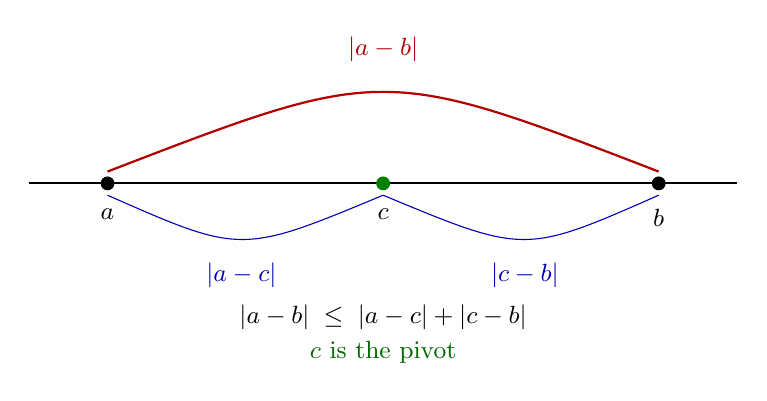
\begin{tikzpicture}[
  dot/.style={circle, fill, inner sep=0pt, minimum size=5pt},
  lbl/.style={font=\small}
]
\draw[thick] (0.5, 0) -- (9.5, 0);
\node[dot] (a) at (1.5, 0) {};
\node[dot, fill=green!50!black] (c) at (5.0, 0) {};
\node[dot] (b) at (8.5, 0) {};
\node[lbl, below] at (1.5, -0.2) {$a$};
\node[lbl, below] at (5.0, -0.2) {$c$};
\node[lbl, below] at (8.5, -0.2) {$b$};
\draw[red!70!black, thick]
  (1.5, 0.15) .. controls (5.0, 1.5) .. (8.5, 0.15);
\node[lbl, above, text=red!70!black] at (5.0, 1.42) {$|a-b|$};
\draw[blue!70!black]
  (1.5, -0.15) .. controls (3.2, -0.9) .. (5.0, -0.15);
\node[lbl, below, text=blue!70!black] at (3.2, -0.88) {$|a-c|$};
\draw[blue!70!black]
  (5.0, -0.15) .. controls (6.8, -0.9) .. (8.5, -0.15);
\node[lbl, below, text=blue!70!black] at (6.8, -0.88) {$|c-b|$};
\node[lbl] at (5.0, -1.7) {$|a-b| \;\leq\; |a-c| + |c-b|$};
\node[lbl, text=green!40!black] at (5.0, -2.15) {$c$ is the pivot};
\end{tikzpicture}
\end{center}
\captionof{figure}{%
  The triangle inequality in distance form. The direct distance $|a-b|$
  (red) is bounded above by the sum of indirect distances $|a-c|$ and
  $|c-b|$ (blue) through pivot $c$. In analysis, $c$ is chosen to split
  $|a-b|$ into two pieces each controlled by a separate hypothesis.%
}
\label{fig:triangle-inequality-pivot}
\medskip
